\section{Démonstration de l'application}
\begin{figure}[h!]
   \begin{minipage}[b]{0.37\linewidth}
      \centering 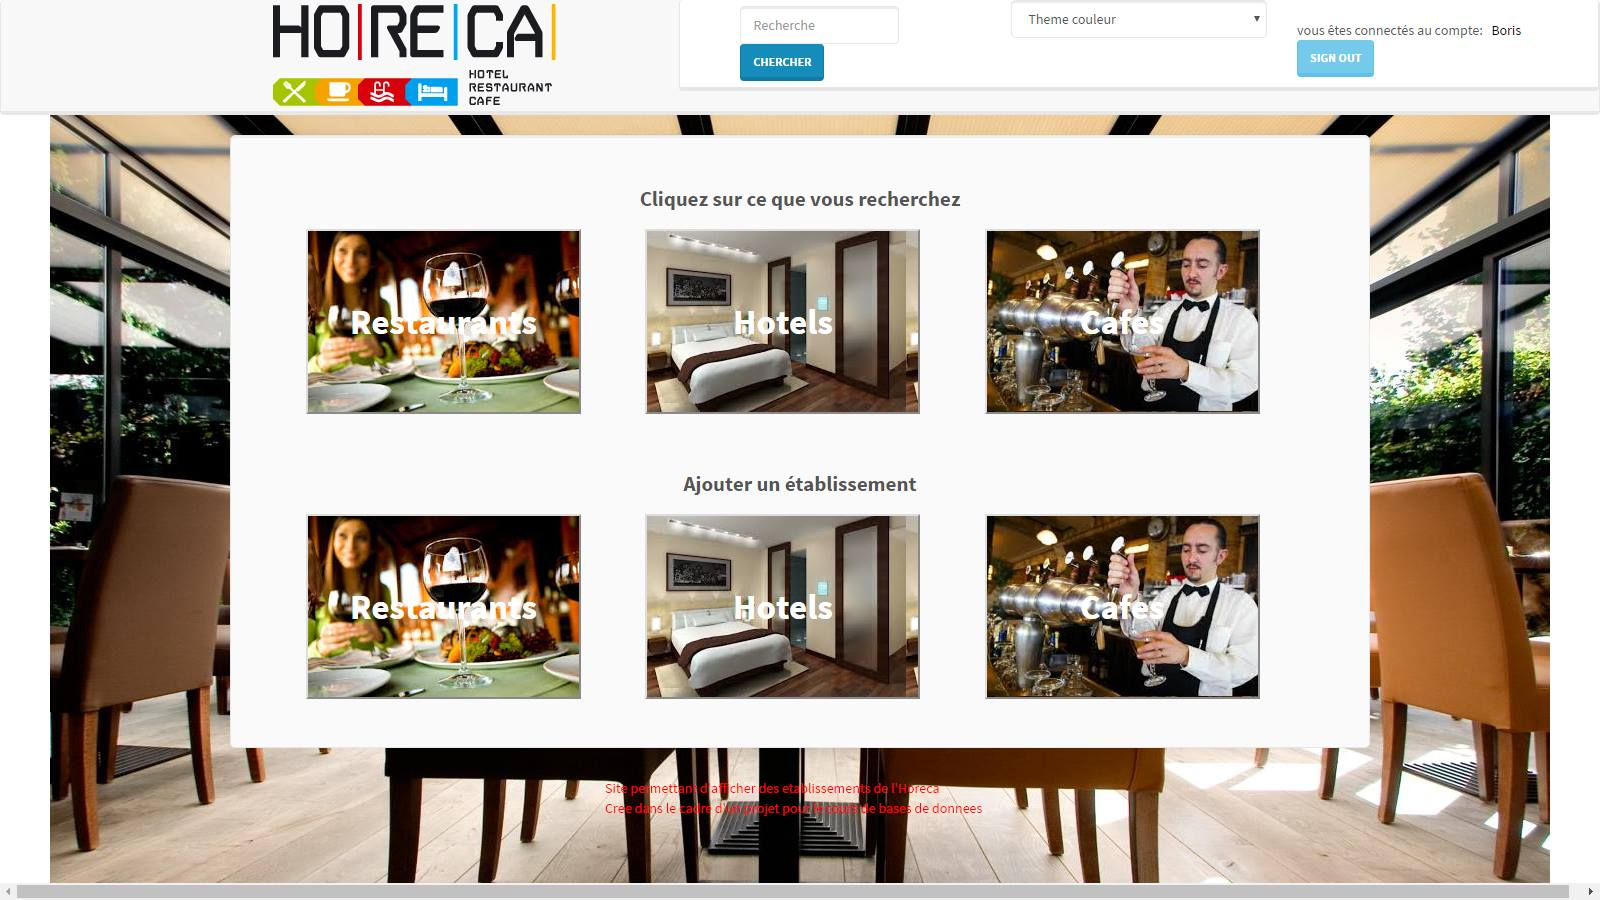
\includegraphics[scale=0.15]{pagegarde}
   \end{minipage}\hfill
   \begin{minipage}[b]{0.37\linewidth}   
      \centering 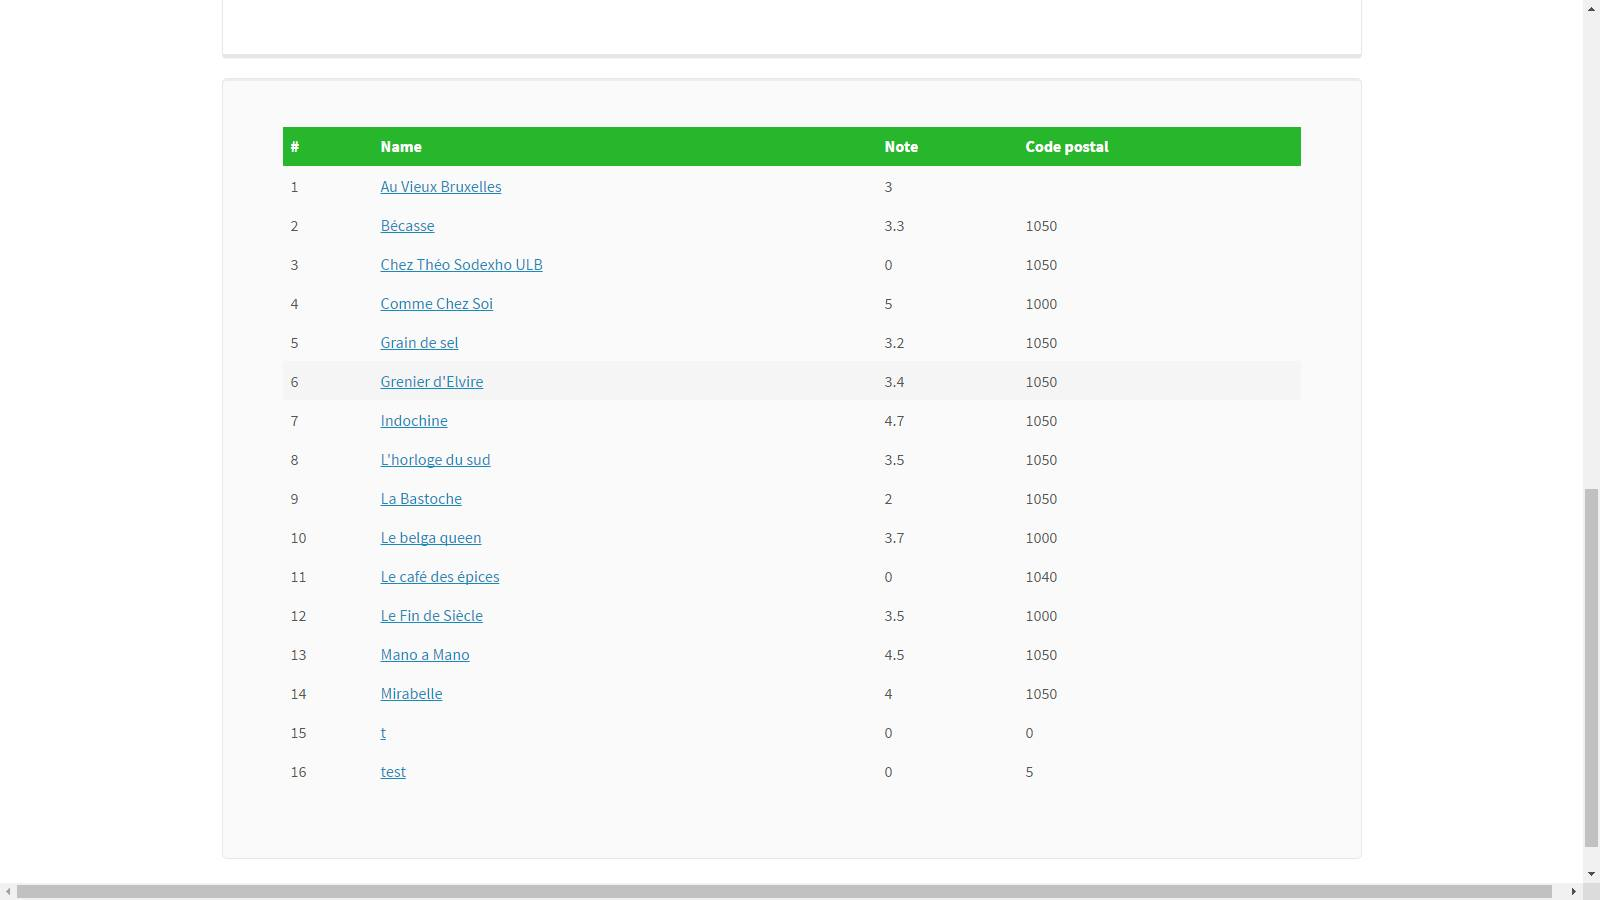
\includegraphics[scale=0.15]{liste}
   \end{minipage}
   \begin{minipage}[b]{0.35\linewidth}
      \centering 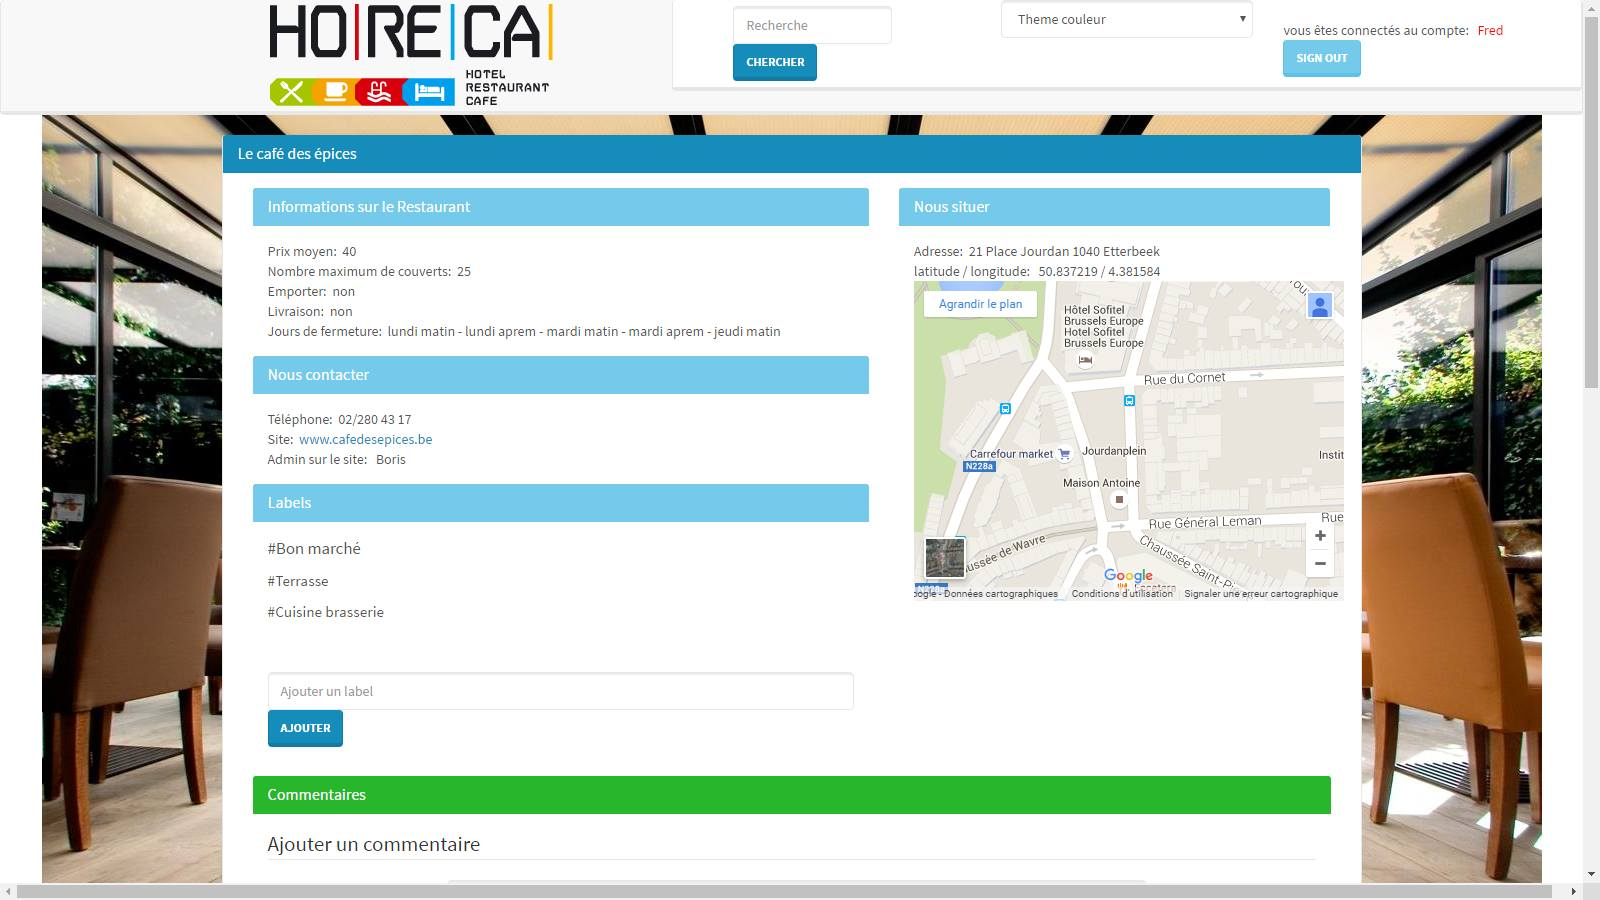
\includegraphics[scale=0.15]{pres}
   \end{minipage}\hfill
   \begin{minipage}[b]{0.35\linewidth}   
      \centering 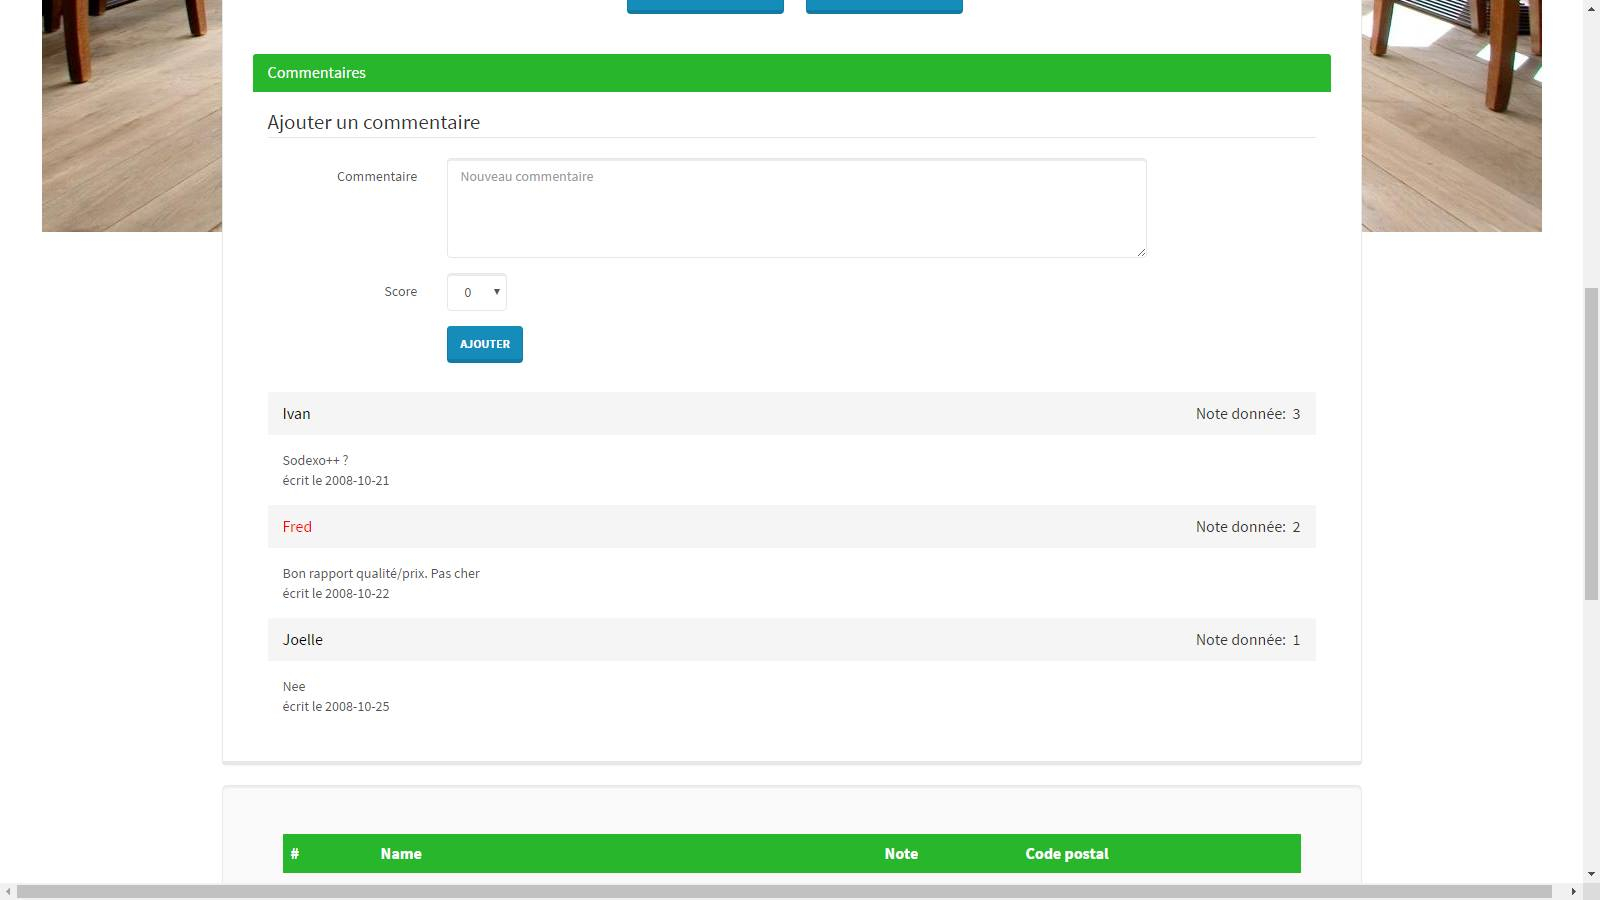
\includegraphics[scale=0.15]{com}
   \end{minipage}
\end{figure}
\noindent Voici une scénario de démonstration de l'application. Considérant que l'utilisateur s'est connecté en tant que administrateur. Celui-ci est amené sur la page de garde où il peut soit créer un nouvel établissement, soit consulter les établissements déjà existant. Après avoir choisi quel type d'établissement il souhaite consulter, il peut choisir quel établissement il veut voir. En cliquant sur le nom de celui-ci, il peut consulter sa fiche détaillée, ses commentaires et ses labels.